\section{What must be in a direct decision representation?}
\label{sec:repr}

This section answers RQ1 and RQ2. \Cref{sec:repr:blind} shows that a candidate-blind decision state
does not preserve question-conditioned capability; \Cref{sec:repr:readout} shows that a
contextual-candidate readout does; \Cref{sec:repr:depth} and \Cref{sec:repr:null} isolate the two
design choices that readout needs to work. Unless noted otherwise, JevBench numbers follow the
disclosures of \Cref{sec:experiments:jevbench} (public 231-id subset, unranked, probabilities
conditioned on non-$\nullsym$).

\subsection{Candidate-blind decision states do not preserve question-conditioned capability}
\label{sec:repr:blind}

\Cref{fig:deltaq} is the paper's central negative result and the reason for everything that follows.
The $x$-axis is raw accuracy on a 1{,}200-item MMLU-Pro among-$\numcands$ knowledge probe; the $y$-axis
is $\dqsh$ (\Cref{def:deltaq}). Every candidate-blind variant we trained lands in the $\pm.02$ band
around zero, and four of the six are \emph{below} zero: the real question buys them nothing over a
shuffled, unrelated one with the candidate set held fixed. Their above-chance accuracy of .12--.17 is
candidate-set priors baked into the corpus.

\begin{figure}[t]
  \centering
  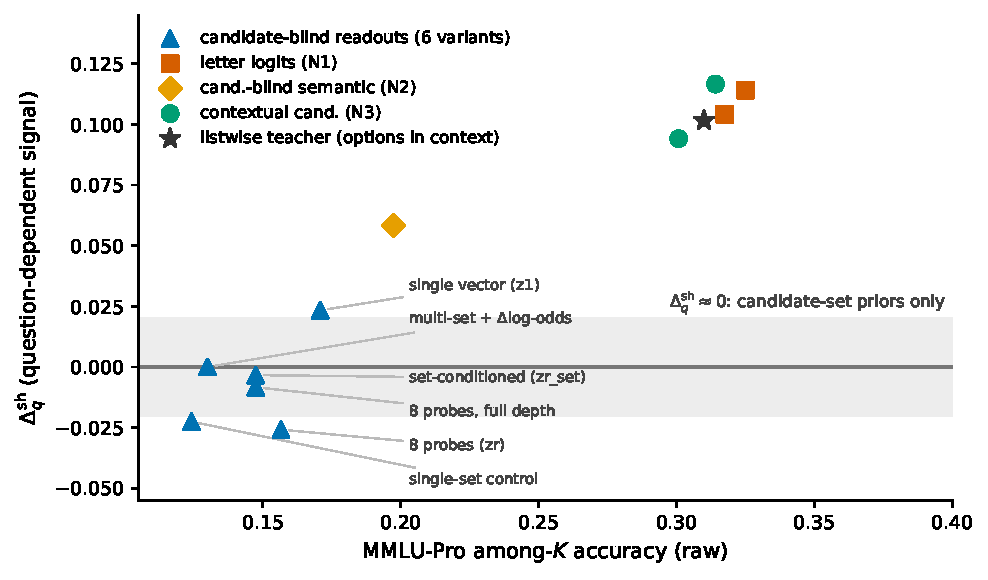
\includegraphics[width=\linewidth]{figures/fig_deltaq.pdf}
  \caption{The candidate-blind negative. Raw MMLU-Pro among-$K$ accuracy against $\dqsh$, the drop in
  accuracy when the real question is replaced by a shuffled one with the candidate set held fixed
  ($n{=}1{,}200$ items; the shaded band is the $\pm.02$ indistinguishable-from-zero region of
  \Cref{sec:experiments:deltaq}). All six candidate-blind variants sit in that band regardless of head
  capacity, set conditioning, objective, or tap depth. The letter-logit readout, the
  contextual-candidate readout, and the listwise teacher all carry a question-dependent signal of
  .09--.12. Raw accuracy alone cannot tell these two groups apart.}
  \label{fig:deltaq}
\end{figure}

\begin{table}[t]
  \centering
  \caption{Candidate-blind students: six factorizations and objectives, two tap depths. ``Shuffled''
  replaces the real question with an unrelated one, candidate set fixed. $\dqsh$ is the difference.
  $n{=}1{,}200$ MMLU-Pro items; $\pm.02$ is the indistinguishable-from-zero band.}
  \label{tab:blind}
  \small
  \begin{tabular}{llrrr}
    \toprule
    Student & Factorization / objective & among-$\numcands$ & shuffled & $\dqsh$ \\
    \midrule
    \texttt{z1} & single decision vector, bilinear scorer & .171 & .147 & $+.023$ \\
    \texttt{zr} & 8 probes, token-level max-similarity & .157 & .182 & $-.026$ \\
    \texttt{zr\_set} & + $O(\numcands)$ cross-attention over candidate tokens & .147 & .151 & $-.003$ \\
    \texttt{ms\_ctrl} & single-set KD, steps-matched control & .124 & .147 & $-.023$ \\
    \texttt{ms\_zr\_set} & same-$Z$ multi-set, explicit $\Delta$log-odds targets & .130 & .130 & $+.000$ \\
    \texttt{zr} (full depth) & 8 probes, tapped at layer 28/28 & .147 & .156 & $-.008$ \\
    \midrule
    Teacher & listwise decoder, options in context & .310 & .208 & $\mathbf{+.102}$ \\
    \bottomrule
  \end{tabular}
\end{table}

\Cref{tab:blind} gives the variants. The negative survives every lever we had. \emph{Head capacity} is
not the bottleneck: a single decision vector retains as much as eight probes. \emph{Set conditioning}
is not the bottleneck: adding $O(\numcands)$ cross-attention over candidate tokens changes nothing on
this axis (it does improve null quality, \Cref{sec:repr:null}). \emph{Supervision} is not the
bottleneck: an explicit same-$Z$ multi-set objective that supervises the \emph{difference} in log-odds
a candidate-set edit induces in the teacher reproduces the teacher's $\Delta$ no better than its own
steps-matched single-set control, and its $\dqsh$ is exactly zero. And \emph{tap depth} is not the
bottleneck: re-running the strongest student at full backbone depth, after depth turned out to be
decisive for the candidate-\emph{aware} readout (\Cref{sec:repr:depth}), leaves $\dqsh$ at $-.008$ while
among-$\numcands$ accuracy \emph{falls} to .147 and every evidence task regresses in the pattern a
last-layer tap predicts (SNLI/MNLI/ANLI/BoolQ .881/.807/.462/.712 at full depth vs.\ .905/.873/.541/.826
at tap 20; \Cref{tab:app-blind-closure}). No further candidate-blind variants were run after this
closure.

What \emph{does} transfer into a candidate-blind state is worth stating precisely, because it is why
accuracy hides the failure: the students inherit the teacher's candidate priors and its calibration.
Expected calibration error on the knowledge probe improves from .39 for an earlier baseline to .04, and
the students are exactly set-stable where the teacher is set-fragile. A reader looking only at accuracy
and ECE would conclude the factorization works.

\textbf{Scope.} This is a scoped empirical result, not an impossibility theorem. It covers the
factorizations, objectives, depths, teacher, and budget listed above, at one backbone family and 1.7B
with 12k steps. Two alternative explanations we cannot exclude: the set-conditioning path's
zero-initialized cross-attention stayed inert over 4k steps, so an optimization failure is a live
alternative to an information-theoretic one; and the teacher's own question-dependent component is
small (.102), so the measurement has roughly nine points of dynamic range. What the result does
establish is a design boundary we then acted on -- and the diagnostic, $\dq$, transfers to any
candidate-scoring architecture whether or not our particular negative does.

\subsection{Contextual-candidate readout recovers the signal}
\label{sec:repr:readout}

We compare three non-generative readouts of the same decision pass, all with candidates rendered in the
suffix: the \textbf{letter-logit readout} (N1: next-token probability over the rendered option letters
-- the ordinary multiple-choice interface, read directly rather than generated); the
\textbf{candidate-blind semantic readout} (N2: a bilinear score between the terminal state $\hD$ and an
independently computed semantic embedding of the option text); and the \textbf{contextual-candidate
readout} (N3, \Cref{sec:method:pass}: a bilinear score between $\hD$ and each option's own contextual
hidden state $\hctx{j}$).

The ordering is the interface-level result. Replacing the option's contextual state with an independent
semantic embedding of the same text costs 13 points of knowledge-probe accuracy (N2 .198 vs.\ N1 .325)
and roughly half the question-dependent signal ($\dqsh$ .058 vs.\ .114). This is not the candidate-blind
failure of \Cref{sec:repr:blind} -- N2 still runs the candidates through the language model and keeps a
real $\dqsh$ -- it is a narrower statement about the readout: an independently embedded candidate is
measurably insufficient even when the candidates are in the computation. \Cref{tab:n1n3} then gives the
matched two-seed comparison between the letter-logit and contextual-candidate readouts.

\begin{table}[t]
  \centering
  \caption{Letter-logit (N1) vs.\ contextual-candidate (N3) readout, two seeds each (identical config,
  \texttt{seed=0} vs.\ \texttt{seed=1}), full-depth backbone (28 layers). Teacher = a fine-tuned decoder
  reading options in context. $\dqsh$ is the shuffled-question variant of \Cref{def:deltaq}.}
  \label{tab:n1n3}
  \small
  \setlength{\tabcolsep}{4pt}
  \begin{tabular}{lrrrrr}
    \toprule
    & N1 seed 0 & N1 seed 1 & N3 seed 0 & N3 seed 1 & Teacher \\
    \midrule
    $\dqsh$ (primary) & .114 & .104 & .117 & .094 & .102 \\
    MMLU-Pro among-$\numcands$ & .325 & .318 & .314 & .301 & .310 \\
    SNLI & .838 & .831 & .863 & .851 & -- \\
    MNLI & .684 & .664 & .752 & .719 & -- \\
    ANLI & .377 & .393 & .431 & .437 & -- \\
    BoolQ & .769 & .764 & .737 & .746 & -- \\
    Reorder max $\Delta p$ & .165 & .165 & .101 & .109 & 0 \\
    Pairwise $\Delta$log-odds & .463 & .443 & .126 & .094 & 0 \\
    \bottomrule
  \end{tabular}
\end{table}

N1 and N3 land within seed noise of each other and of the teacher on $\dqsh$ (N1 mean .109, N3 mean
.106, teacher .102): the contextual-candidate readout preserves essentially all of the letter
interface's question-conditioned signal while generating nothing. It does so with roughly a quarter of
the letter interface's order sensitivity (reorder $\Delta p$ .10--.11 vs.\ .165; pairwise
$\Delta$log-odds under candidate-set edits .09--.13 vs.\ .44--.46) and a consistent evidence-task
advantage (SNLI $+2$, MNLI $+6$--$7$, ANLI $+4$--$5$ points, both seeds). Two honest caveats: the
equivalence claim sits at the noise floor -- the seed spread on $\dqsh$ is .01--.02 and the claimed gap
is .003, so this is ``indistinguishable at two seeds'', not a demonstrated equality -- and order
sensitivity is \emph{reduced}, not eliminated; a permutation-invariant candidate-blind scorer gets
exactly zero, so the honest position is that the contextual readout sits between the letter interface
and a set-invariant scorer. Both arms train with per-step option shuffling, so part of the robustness is
augmentation rather than architecture.

\subsection{Why intermediate depth}
\label{sec:repr:depth}

Depth is the one lever that separates the two readouts, and it separates them in opposite directions.
Reading the contextual-candidate readout at the tap-20 truncation rather than the full 28-layer backbone
recovers evidence-task accuracy to within 1--3 points of a candidate-blind energy baseline on every
evidence set (and $+8$ points on CLINC-150) while \emph{keeping} the question-conditioned signal ($\dqsh$
.118 at tap 20 vs.\ .117 at full depth, $1.16\times$ the teacher's). At the last layer the same readout
loses 5--15 points of evidence accuracy relative to that baseline. For the candidate-blind state, the
same depth change does nothing to $\dqsh$ at all (\Cref{sec:repr:blind}).

The conceptual point is more interesting than the flag: the final representation of a causal LM is
optimized for next-token prediction, and it is not automatically the best representation for an
evidence-grounded direct decision. Once the options are rendered inside the suffix, reading an
intermediate layer is required to recover the backbone's pretrained evidence reasoning. That
mid-depth features can beat last-layer features for classification is itself established
\citep{gromov2024deeperlayers,men2024shortgpt,tenney2019pipeline,belrose2023tunedlens}; what is specific
here is that the choice is decisive for a deployed decision interface and interacts with the readout,
not with the backbone. We chose one tap fraction (71\%) and ported it across backbone sizes without a
per-size sweep, which is a limitation.

\subsection{Abstention: a rendered abstain option is a softmax-dilution bug}
\label{sec:repr:null}

An early model rendered a literal ``none of the above'' line as one more option in the suffix and let it
compete for softmax mass. This has a $\numcands$-dependent pathology: the abstain option's share
dilutes as the candidate set grows, whether or not the true label is absent. Replacing it with the
factored gate of \Cref{eq:factored-null} fixes that essentially for free (\Cref{tab:app-null-fix}): the
$\numcands$-sweep of null AUROC becomes monotone, MMLU-Pro false-abstention drops from .692 to .003 with
accuracy rising from .133 to .353, and Banking77 goes from unusable (.063) to .579 -- with $\dqsh$
unchanged (.118 vs.\ .122) and evidence tasks at the same level. The remaining costs are smaller and
specific: intent/topic label spaces lose 2--7 points and order sensitivity rises slightly, because with
no rendered null line the letter position is the only identity signal left in the suffix.

Three things that are easy to conflate should stay separate. The \emph{rendered-null pathology} is a
rendering artifact. The \emph{exact pairwise non-null odds} property is an algebraic consequence of the
factorization (\Cref{sec:method:typed}). \emph{Null calibration across $\numcands$} is a measured
property that the factorization makes achievable but does not guarantee -- and it is partly a property
of our training mixture, since under 1\% of workflow rows naturally carry a null target, which is why
null augmentation exists (\Cref{sec:method:mixture}). This is also the single-model, no-workflow-training
configuration that scores .694 standard / .378 hard on JevBench (public subset, unranked) and is the
base for every workflow-trained checkpoint in \Cref{sec:train}.
